\chapter{Návrh funkcionality}
	Ďalej opíšeme ako je naše riešenie navrhnuté. Popíšeme ako budeme postupovať v prípade nahrávania, sťahovania, zdieľania a čo spravíme keď už nechceme zdieľať dáta. Potom si popíšeme, čo treba spraviť predtým, ako budeme môcť tieto akcie vykonať.
	
	\section{Prerekvizity}
	
		Aby naše riešenie fungovalo, budeme potrebovať server, ktorý bude poskytovať API na komunikáciu s databázou a bude hostovať naše webové rozhranie. Databázu kam budeme ukladať užívateľove kľúč a kľúče k súborom. Cloudové úložisko, ktoré bude zabezpečovať prácu so súbormi. Cloud musí poskytovať rozhranie pomocou ktorého vieme nahrávať a sťahovať dáta a taktiež musí byť schopné autorizovať rôznych užívateľov pre prístup k dátam iných užívateľov, aby sme mohli zdieľať súbory s inými používateľmi. 
		
	\section{Registrácia}
		
		Keď sa používateľ rozhodne používať našu službu musí sa nejakým spôsobom identifikovať a autentifikovať. Identifikácia vyžaduje aby si každý používateľ zvolil nejaké meno a aby sme ho mohli authentifikovať potrebuje heslo. Druhou možnosťou je využiť tretiu službu ako napríklad cloud kde budeme ukladať súbory. Toto je možné napríklad pomocou protokolov oAuth alebo openID. Nech už vybereme jeden alebo druhý spôsob budeme jednoznačne vedieť s kým komunikujeme. S touto informáciou vyzveme užívateľa aby si zvolil svoje univerzálne heslo pomocou ktorého bude autorizovať akcie ako nahrávanie, sťahovanie, zdieľanie a zrušenie zdieľania dát.
		\\Následne v užívateľovom prehliadači vygenerujeme verejný a privátny kľúč, ktorý symetricky zašifrujeme pomocou už zvoleného univerzálneho hesla. Verejný aj zašifrovaný privátny kľúč uložíme na serveri kde prístup k verejným kľúčom budú mať všetci používatelia no k privátnym len jeho vlastníci. Tým že privátny kľúč je zašifrovaný server nemá žiadnu informáciu o privátnom kľúči a teda schéma ostane bezpečná. 
		\\Ďaľšou možnosťou bolo uložiť privátny kľúč na užívateľovom počítači. Toto sme sa rozhodli nevyužiť z dôvodu náročného manažmentu kľúčov na rôznych zariadeniach. Napríklad pri strate zariadenia by to vyžadovalo zmenu privátneho kľúču, čo by implikovalo nutnosť prešifrovania všetkých súborových kľúčov. Poprípade distribúcia kľúču do rôznych zariadení by bola v rukách používateľa čo by mohlo byť nepohodlnné.
		
		
		\begin{figure}[H]
			\begin{center}
				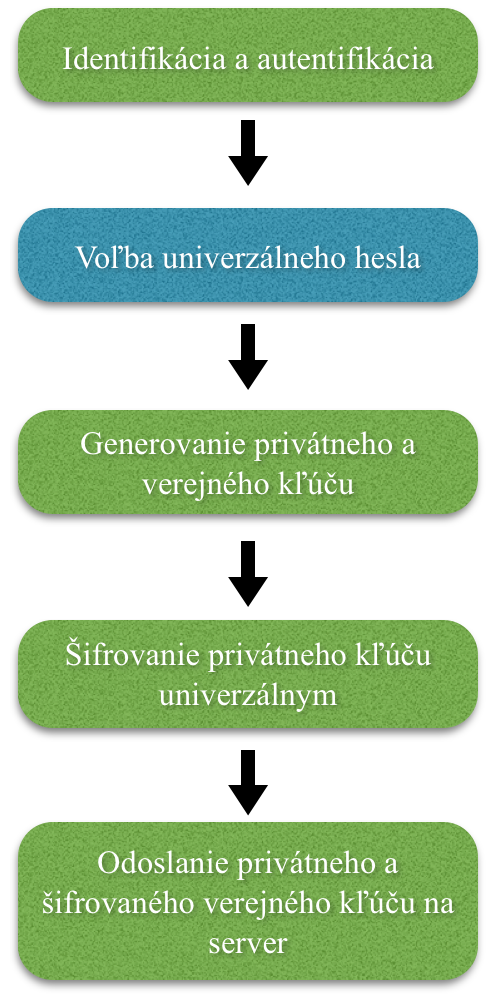
\includegraphics[width=0.5\linewidth]{images/registracia.png}
				\caption{Priebeh registracie }
			\end{center}
		\end{figure}
		
	
	\section{Nahrávanie dát}
	
		Užívateľ sa authentifikuje a v prehliadači a pomocou pseudonáhodného generátoru vygeneruje náhodný text. Ten využije ako heslo, s ktorým zašifruje súbor a vypýta si od servera svoj verejný kľúč. Pomocou verejného kľúču zašifruje heslo k súboru a v taktomto tvare ho už môže poslať na server. Keďže heslo je zašifrované a server nemá žiadnu informáciu o privátnom kľúči, nevie získať dáta v otvorenom tvare. Následne už len stačí zašifrovaný súbor nahrať na cloudové úložisko.
		
		\begin{figure}[H]
			\begin{center}
				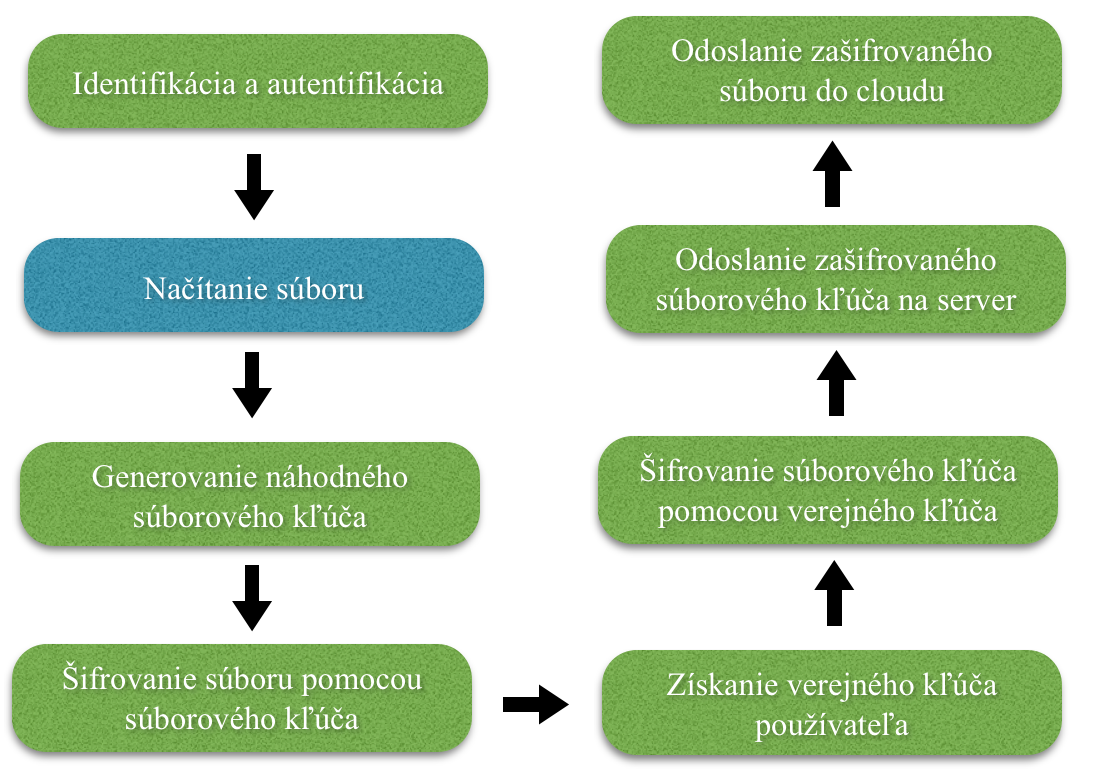
\includegraphics[width=1\linewidth]{images/nahravanie.png}
				\caption{Nahrávanie dát}
			\end{center}
		\end{figure}
				
	\section{Sťahovanie dát}
	
		V prípade, že privátny kľúč je uložený na serveri, tak si ho vypýtame a požiadame užívateľa o jeho univerzálne heslo, aby sme mohli privátny kľúč dešifrovať. S privátnym kľúčom môžeme následne dešifrovať heslo k súboru, ktoré si opäť vypýtame od servera. V tejto chvíli máme k dispozícii kľúč k súboru a teda nám stačí stiahnuť súbor z cloudu a rozšifrovať ho pomocou zmieneného kľúča. 
		
		\begin{figure}[H]
			\begin{center}
				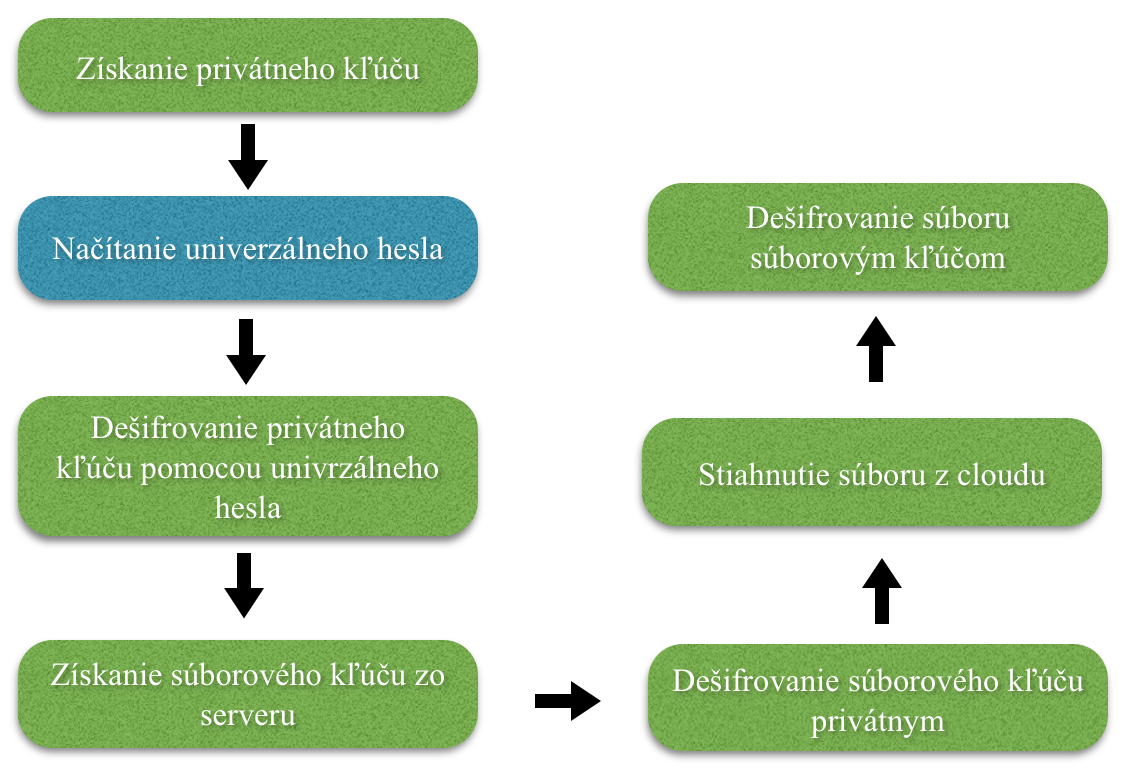
\includegraphics[width=1\linewidth]{images/stahovanie.png}
				\caption{Sťahovanie dát}
			\end{center}
		\end{figure}	
		
	\section{Zdieľanie}
	
		Chceme zdieľať súbor ktorý je uložený v zašifrovanej forme na cloude. Na zdieľanie je nutné, aby cieľový príjmatel bol zaregistrovaný na našom serveri a mal vygenerovaný privátny a verejný kľúč. Zdieľanie bude prebiehať tak, že používateľ si od serevra vypýta privátny kľúč, ktorý dešifruje pomocou svojho univerzálneho kľúču. Následne požiada server o zašifrovaný kľúč k súboru, ktorý dešifruje pomocou privátneho kľúču. Dešifrovaný kľúč k súboru potom zašifruje verejným kľúčom používateľa, s ktorým chce dáta zdieľať a takýto kľúč k súboru uloží na serveri. Následne pošle požiadavku na cloud, aby povolil prístup k súboru používateľovi, s ktorým zdieľame. Príjemca nášho zdieľaného súboru má teraz prístup ku kľúču na dešifrovanie súboru a tiež si môže stiahnuť zašifrovaný súbor z cloudu.
		
		\begin{figure}[H]
			\begin{center}
				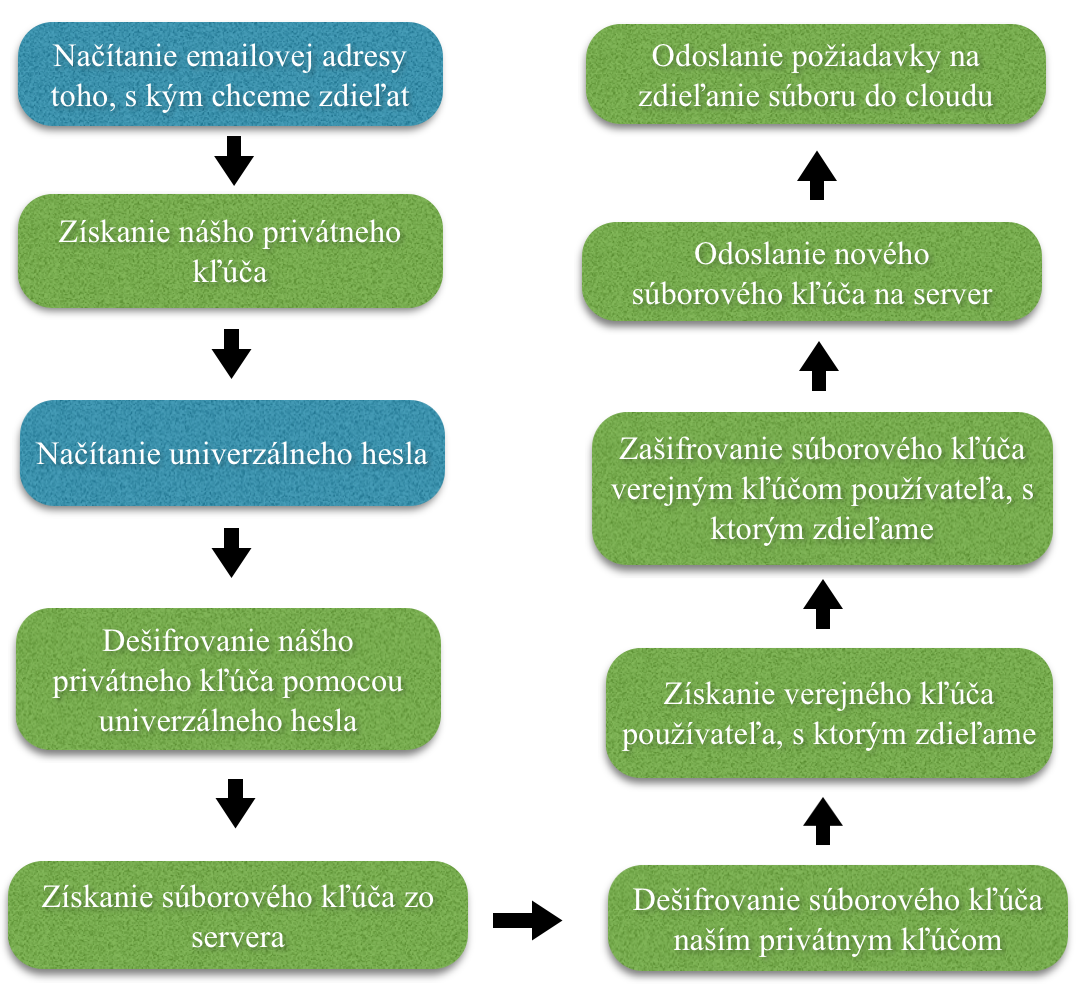
\includegraphics[width=1\linewidth]{images/zdielanie.png}
				\caption{Zdieľanie dát}
			\end{center}
		\end{figure}
		
	\section{Zrušenie zdieľania}
	
		V prípade, že sa rozhodneme zrušiť zdieľanie súboru, stačí, aby sme požiadali cloudové úložisko o revokovanie prístupu k súborom. Keby sa používateľ, s ktorým ten súbor zdieľame, rozhodol ho zverejniť alebo inak distribuovať, šifrovanie nám nepomôže, pretože už si mohol spraviť kópiu nešifrovanej verzie. Preto stačí revokovať prístup na cloude a nemusíme súbor prešifrovať. V prípade, že sa súbor zmení a budeme ho znova uploadovať prebehne opäť procedúra ako pri nahrávaní dát. Nové informácie teda nebudú kompromitované.
	